\documentclass[11pt,a4paper]{article}
\usepackage[T1]{fontenc}
\usepackage{lmodern}
\usepackage{microtype}
\usepackage[margin=2.5cm]{geometry}
\usepackage{parskip}
\usepackage{amsmath,amssymb}
\usepackage{graphicx}
\usepackage{longtable,booktabs}
\usepackage{enumitem}
\setlist{nosep}
\newlist{checklist}{itemize}{1}
\setlist[checklist]{label=$\square$}
\usepackage{xcolor}
\usepackage{listings}
\usepackage[most]{tcolorbox}
\usepackage{xurl}
\usepackage[hidelinks]{hyperref}

\setcounter{secnumdepth}{2}
\setcounter{tocdepth}{2}
\emergencystretch=3em

\lstset{
  basicstyle=\ttfamily\small,
  backgroundcolor=\color{black!5},
  frame=none,
  columns=fullflexible,
  keepspaces=true,
  upquote=true,
  breaklines=true,
  showstringspaces=false,
  commentstyle=\color{black!55},
  keywordstyle=\color{blue!60!black},
  stringstyle=\color{green!40!black},
}

\newtcolorbox{note}{enhanced, breakable, colback=white, colframe=blue!70,
  leftrule=0.75mm, toprule=0.15mm, rightrule=0.15mm, bottomrule=0.15mm,
  arc=0.35mm, title={Note}, coltitle=black, colbacktitle=blue!8}
\newtcolorbox{tip}{enhanced, breakable, colback=white, colframe=green!60!black,
  leftrule=0.75mm, toprule=0.15mm, rightrule=0.15mm, bottomrule=0.15mm,
  arc=0.35mm, title={Tip}, coltitle=black, colbacktitle=green!8}
\newtcolorbox{wip}{enhanced, breakable, colback=white, colframe=yellow!80!black,
  leftrule=0.75mm, toprule=0.15mm, rightrule=0.15mm, bottomrule=0.15mm,
  arc=0.35mm, title={Work in progress}, coltitle=black, colbacktitle=yellow!25}

\title{UAV Research Onboarding\\[0.5ex]
  \large Linux, Git, ROS 2, PX4 and Gazebo, for master's thesis students at
  Politecnico di Torino}
\author{Riccardo Enrico}
\date{}

\begin{document}
\maketitle
\begin{abstract}
This guide teaches the minimum you need to start work in a UAV research
group. It assumes you have never used Linux, Git, ROS 2, PX4 or Gazebo.
It covers only the tools a typical group uses: Ubuntu,
ROS 2, PX4 firmware with Gazebo simulation, Isaac Sim, and a ground
station. Read it once, then use the
\hyperref[first-day-checklist]{First-day checklist} on your first day.
\end{abstract}

\tableofcontents

\section{Versions}\label{versions}

Everything below targets these versions. When the group upgrades, change
this table and check the commands that mention a version.

\begin{longtable}{@{}p{0.232\linewidth} p{0.232\linewidth} p{0.476\linewidth}@{}}
\toprule
Component & Version & Note \\
\midrule
Ubuntu & 24.04 & the only supported Linux; do not install 26.04, even
though it is the newest LTS: ROS 2 Jazzy targets 24.04. Check with
\texttt{lsb\_release -a} \\
ROS 2 & Jazzy & docs:
\href{https://docs.ros.org/en/jazzy}{docs.ros.org/en/jazzy} \\
PX4 firmware & 1.17 & docs: use the page for 1.17 \\
\texttt{px4\_msgs} & branch \texttt{release/1.17} & must match the
firmware \\
Gazebo & Harmonic (\texttt{gz}) & as installed by the PX4 setup
script \\
Micro XRCE-DDS Agent & as installed in the lab &
\texttt{MicroXRCEAgent} \\
QGroundControl & current stable & ground station \\
Isaac Sim & ask your supervisor & see \hyperref[isaac-sim]{Isaac Sim} \\
\bottomrule
\end{longtable}

\section{Linux}\label{linux}

\subsection{The terminal and the
filesystem}\label{the-terminal-and-the-filesystem}

Almost all work happens in a terminal. You type a command, press Enter,
and read the output. The shell (here \texttt{bash} or \texttt{zsh}) is
the program that reads your commands.

Linux has one directory tree that starts at \texttt{/} (the root). Your
own files live in your home directory, written
\texttt{\textasciitilde{}} (for example \texttt{/home/riccardo}). A
\emph{path} says where a file is. An \emph{absolute} path starts with
\texttt{/} or \texttt{\textasciitilde{}}. A \emph{relative} path starts
from the current directory. The path \texttt{.} is the current directory
and \texttt{..} is its parent.

\begin{figure}[htbp]
\centering
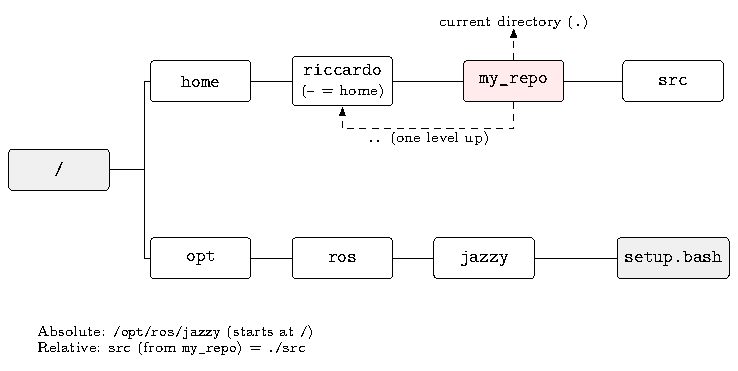
\includegraphics[width=0.8\linewidth]{figures/fs_tree}
\caption{One directory tree, rooted at \texttt{/}. \texttt{\textasciitilde{}} is your home directory, \texttt{.} the current directory and \texttt{..} its parent.}
\end{figure}

\begin{lstlisting}[language=bash]
pwd                       # print the current directory
ls -l                     # list files, one per line, with details
cd ~/my_repo              # change directory
cd ..                     # go to the parent directory
mkdir -p ws/src           # make a directory (and parents)
cp a.txt b.txt            # copy;   mv a.txt c.txt  moves or renames
rm b.txt                  # delete a file (no recycle bin!)
cat file.txt              # print a file;  less file.txt  to scroll
grep -rn "offboard" src/  # search text in files
man ls                    # manual page of a command (q to quit)
\end{lstlisting}

Tips: press Tab to complete names. Press the up arrow to recall old
commands. Press Ctrl-R to search your history. File names are case
sensitive.

\subsection{Permissions and sudo}\label{permissions-and-sudo}

Each file has an owner and three permission sets: owner, group, others.
Each set allows read (\texttt{r}), write (\texttt{w}) and execute
(\texttt{x}). \texttt{ls -l} shows them, for example
\texttt{-rwxr-xr-x}. A script must have the execute bit to run as
\texttt{./script.sh}.

\begin{lstlisting}[language=bash]
chmod +x script.sh        # make a file executable
sudo apt update           # run one command as administrator
\end{lstlisting}

Use \texttt{sudo} only when a command needs it (installing system
packages). Never run ROS or your own code with \texttt{sudo}.

\subsection{Environment variables and
source}\label{environment-variables-and-source}

An environment variable is a named string that programs can read. ROS 2
depends on them. Print one with \texttt{echo \$ROS\_DISTRO}. Set one
for the current shell with \texttt{export ROS\_DOMAIN\_ID=7}.

A setup file such as \texttt{/opt/ros/jazzy/setup.bash} sets many
variables at once (it extends \texttt{PATH}, the list of folders where
the shell looks for programs). You must \emph{source} it, not run it:

\begin{lstlisting}[language=bash]
source /opt/ros/jazzy/setup.bash
\end{lstlisting}

Sourcing changes only the current terminal. When you open a new terminal
you must source again, or put the line in
\texttt{\textasciitilde{}/.bashrc} (read at the start of every bash
terminal). A frequent beginner error is ``command not found'' for
\texttt{ros2} or \texttt{colcon}: you forgot to source.

\begin{note}
If your shell is \texttt{zsh}, source the \texttt{.zsh} file instead
(\texttt{/opt/ros/jazzy/setup.zsh}) and put the line in
\texttt{\textasciitilde{}/.zshrc}.
\end{note}

\begin{tip}
Put the base ROS 2 setup file (\texttt{setup.bash} or
\texttt{setup.zsh}) in your shell startup file. Source the overlay of
your workspace (\texttt{install/setup.bash}) only when you work in that
workspace (\hyperref[workspaces-and-colcon]{Workspaces and colcon}).
\end{tip}

\subsection{Installing software with
apt}\label{installing-software-with-apt}

Ubuntu installs system software with \texttt{apt}.

\begin{lstlisting}[language=bash]
sudo apt update                        # refresh the package list
sudo apt install git build-essential   # install packages
apt search ros-jazzy-rqt               # search
\end{lstlisting}

\subsection{Processes}\label{processes}

Every running program is a process. Press Ctrl-C in a terminal to stop
the program in it. Ctrl-Z suspends it. If a program hangs, or a
simulator stays alive in the background:

\begin{lstlisting}[language=bash]
ps aux | grep -i gz        # find processes whose line contains "gz"
kill 12345                 # ask process 12345 to stop (12345 is the PID)
kill -9 12345              # force it, if the first kill did not work
pkill -f px4               # kill by name pattern
htop                       # live process viewer (q to quit)
\end{lstlisting}

You will run several programs at once (the simulator, the bridge to PX4,
your own nodes). Use one terminal for each, or a terminal multiplexer
such as \texttt{tmux}.

\subsection{SSH into the onboard
computer}\label{ssh-into-the-onboard-computer}

The drone carries a small computer. You log in to it over the network
with SSH.

\begin{note}
The lab drones are already set up. Read this section for background, and
use it when you set up new hardware.
\end{note}

\begin{lstlisting}[language=bash]
ssh-keygen -t ed25519              # once: make a key pair
ssh-copy-id user@drone-ip          # copy the public key to the drone
ssh user@drone-ip                  # log in; type "exit" to leave
scp file.txt user@drone-ip:~/      # copy a file to the drone
\end{lstlisting}

Ask your supervisor for the user name and the IP address of the
onboard computer; they are not written here on purpose. The same key
type is used to push to GitHub (\hyperref[git-and-github]{Git and
GitHub}).

\subsection{Editors}\label{editors}

Use what you like. Recommended editors:

\begin{itemize}
\item
  \href{https://code.visualstudio.com}{VS Code}: the most used in the
  group. Its ``Remote - SSH'' extension edits files on the drone.
\item
  \href{https://zed.dev}{Zed}: built in Rust, faster.
\item
  \href{https://neovim.io}{Neovim}: not beginner friendly.
\end{itemize}

\texttt{nano file} is the simplest terminal editor (Ctrl-O saves,
Ctrl-X exits). If you land in \texttt{vim} by accident, press Esc, then
type \texttt{:q!} and Enter to leave.

\section{Git and GitHub}\label{git-and-github}

Git records the history of a folder (a \emph{repository}). Each saved
state is a \emph{commit}. GitHub hosts a copy of the repository online
and adds issues and pull requests. Lab repositories are usually private.
Ask for access, add your SSH public key
(\texttt{\textasciitilde{}/.ssh/id\_ed25519.pub}) in your GitHub account
settings, and test with \texttt{ssh -T git@github.com}.

\subsection{Daily commands}\label{daily-commands}

\begin{lstlisting}[language=bash]
git clone --recursive git@github.com:<owner>/<repo>.git
cd <repo>
git status                  # what changed?
git diff                    # show the changes in detail
git add src/my_node.cpp     # stage a file for the next commit
git commit -m "feat(controller): add acceleration limit"
git push                    # upload your commits
git pull                    # download and merge new commits
git log --oneline -10       # last 10 commits
\end{lstlisting}

The flow is: edit files, \texttt{git add} the ones that belong
together, \texttt{git commit} with a message, \texttt{git push}. A
commit is local until you push.

\begin{figure}[htbp]
\centering
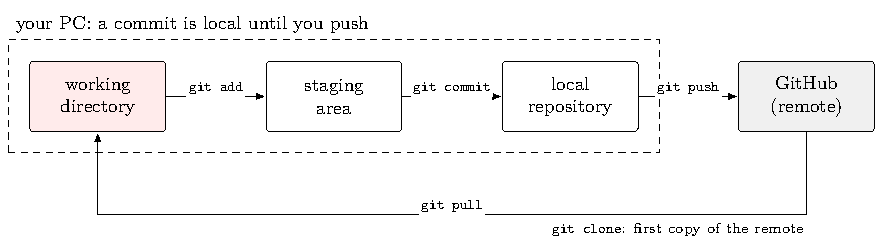
\includegraphics[width=0.95\linewidth]{figures/git_flow}
\caption{\texttt{git add} stages, \texttt{git commit} records locally, and only \texttt{git push} sends the commits to GitHub. \texttt{git pull} brings new commits back.}
\end{figure}

Write commit messages as
\href{https://www.conventionalcommits.org}{Conventional Commits}:
\texttt{\textless{}type\textgreater{}(\textless{}scope\textgreater{}): \textless{}description\textgreater{}},
for example \texttt{feat(controller): add acceleration limit} or
\texttt{fix(bridge): correct frame conversion}.

\subsection{Branches}\label{branches}

A branch is a movable label for a line of commits. Do your work on a
branch, not on \texttt{main}.

\begin{lstlisting}[language=bash]
git switch -c feat/12-hover-node       # make and switch to a new branch
git switch main                        # go back
git push -u origin feat/12-hover-node  # first push of a new branch
\end{lstlisting}

Branch names start with the type (\texttt{feat}, \texttt{fix},
\texttt{docs}, \texttt{chore}) and should contain the issue number.

\begin{figure}[htbp]
\centering
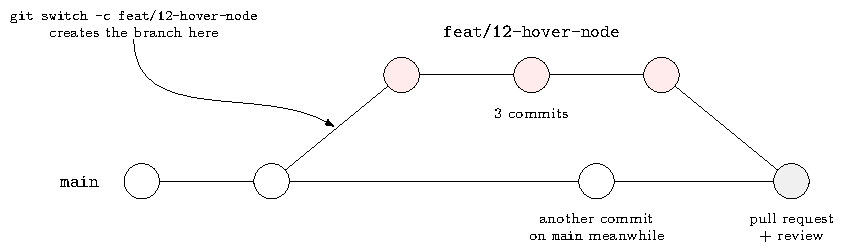
\includegraphics[width=0.9\linewidth]{figures/git_branches}
\caption{\texttt{git switch -c} starts a branch off \texttt{main}. You commit on it, and a reviewed pull request merges it back.}
\end{figure}

\subsection{Commit messages}\label{commit-messages}

Messages follow Conventional Commits:
\texttt{type(scope): description}. Examples:

\begin{lstlisting}
feat(controller): add tilt limit
fix(mapper): clamp negative distance
docs(guide): add ROS 2 section
\end{lstlisting}

Use the imperative, lower case, no final period. Add \texttt{refs \#12}
(or \texttt{fixes \#12}) at the end of the body to link the commit to
an issue.

\subsection{Issues and pull requests}\label{issues-and-pull-requests}

An \emph{issue} describes one task. Check the open issues before you
start, and write one for new work. A \emph{pull request} (PR) asks to
merge your branch into \texttt{main}. Someone reviews it, then it is
merged. If \texttt{git pull} reports a \emph{conflict}, Git marks the
clashing lines with
\texttt{\textless{}\textless{}\textless{}\textless{}\textless{}\textless{}\textless{}};
edit the file to keep what you want, \texttt{git add} it, and
\texttt{git commit}.

\subsection{Submodules}\label{submodules}

A project can include another repository inside it. A typical case in a
PX4 project is the message package:

\begin{longtable}{@{}p{0.225\linewidth} p{0.357\linewidth} p{0.357\linewidth}@{}}
\toprule
Path & Content & Pinned to \\
\midrule
\texttt{src/px4\_msgs} & PX4 message definitions (public) & branch
\texttt{release/1.17} (e.g.~tag \texttt{v1.17.0}) \\
\bottomrule
\end{longtable}

A submodule is pinned to one commit. The parent repo
does not store the files of the submodule. It stores the URL (in
\texttt{.gitmodules}) and one exact commit hash. When you clone, you get
that commit and nothing else, so everyone builds the same code.

\begin{lstlisting}[language=bash]
# add it once, following the firmware's release branch
git submodule add -b release/1.17 \
  https://github.com/PX4/px4_msgs.git src/px4_msgs

# fresh clone with everything, including nested submodules
git clone --recursive git@github.com:<owner>/<repo>.git

# you cloned without --recursive, or someone bumped a submodule:
git submodule update --init --recursive

git submodule status        # shows the pinned hash of each one
\end{lstlisting}

A leading \texttt{+} in the status means the submodule folder is at a
different commit than the parent pins. A leading \texttt{-} means it is
not initialised yet. After a plain \texttt{git pull} in the parent, run
\texttt{git submodule update -\/-init -\/-recursive} so the folders
follow the new pins.

\textbf{Bumping a submodule.} To move \texttt{px4\_msgs} to a newer
commit of its release branch:

\begin{lstlisting}[language=bash]
cd src/px4_msgs
git fetch && git switch release/1.17 && git pull   # get the new commit
cd ../..
git status        # shows: modified: src/px4_msgs (new commits)
git add src/px4_msgs
git commit -m "build: bump px4_msgs"
\end{lstlisting}

Rule: if you change code \emph{inside} a submodule you own, commit and
push it \emph{there first}, then commit the new pin in the parent. If
you do it in the other order, other people cannot fetch the pinned
commit. Do not bump \texttt{px4\_msgs} on your own to a different
release line: it must match the PX4 firmware (\hyperref[px4]{PX4}).

\section{ROS 2}\label{ros-2}

ROS 2 is a set of libraries and tools to build robot software as many
small programs that talk to each other. This guide uses Ubuntu 24.04 and
ROS 2 \textbf{Jazzy} (see \hyperref[versions]{Versions}). Use Jazzy
commands and documentation
(\href{https://docs.ros.org/en/jazzy}{docs.ros.org/en/jazzy}); older
tutorials may differ.

\subsection{Installing ROS 2 Jazzy}\label{installing-ros-2-jazzy}

A new machine has no ROS 2. Check with \texttt{ls /opt/ros}: if the
folder is missing or does not list \texttt{jazzy}, install the deb
packages, following the official
\href{https://docs.ros.org/en/jazzy/Installation/Ubuntu-Install-Debs.html}{Ubuntu
install page}. Do the steps in order and check the output of each
before the next.

\begin{enumerate}
\item
  Check that the locale supports UTF-8 (for example
  \texttt{en\_US.UTF-8}). If it does not, the install page shows how to
  set one.
\begin{lstlisting}[language=bash]
locale
\end{lstlisting}
\item
  Enable the Ubuntu universe repository.
\begin{lstlisting}[language=bash]
sudo apt install software-properties-common
sudo add-apt-repository universe
\end{lstlisting}
\item
  Add the ROS 2 apt repository. One package installs its keys and
  sources. Run these four lines in the same terminal: the second line
  sets a variable that the third line uses.
\begin{lstlisting}[language=bash]
sudo apt update && sudo apt install curl -y
export ROS_APT_SOURCE_VERSION=$(curl -s https://api.github.com/repos/ros-infrastructure/ros-apt-source/releases/latest | grep -F "tag_name" | awk -F'"' '{print $4}')
curl -L -o /tmp/ros2-apt-source.deb "https://github.com/ros-infrastructure/ros-apt-source/releases/download/${ROS_APT_SOURCE_VERSION}/ros2-apt-source_${ROS_APT_SOURCE_VERSION}.$(. /etc/os-release && echo ${UBUNTU_CODENAME:-${VERSION_CODENAME}})_all.deb"
sudo dpkg -i /tmp/ros2-apt-source.deb
\end{lstlisting}
\item
  Update the system. ROS 2 packages are built against an up-to-date
  Ubuntu.
\begin{lstlisting}[language=bash]
sudo apt update && sudo apt upgrade
\end{lstlisting}
\item
  Install ROS 2 and the build tools. \texttt{ros-jazzy-desktop}
  includes RViz, the demos and the tutorials; \texttt{ros-dev-tools}
  brings \texttt{colcon}. If \texttt{ros-dev-tools} fails with
  dependency conflicts, the install page has the fix.
\begin{lstlisting}[language=bash]
sudo apt install ros-jazzy-desktop ros-dev-tools
\end{lstlisting}
\item
  Test the install. In one terminal start a talker:
\begin{lstlisting}[language=bash]
source /opt/ros/jazzy/setup.bash
ros2 run demo_nodes_cpp talker
\end{lstlisting}
  In a second terminal start a listener:
\begin{lstlisting}[language=bash]
source /opt/ros/jazzy/setup.bash
ros2 run demo_nodes_py listener
\end{lstlisting}
  The talker prints \texttt{Publishing} lines and the listener prints
  \texttt{I heard} lines.
\end{enumerate}

\subsection{Installing the other tools}\label{installing-the-other-tools}

A new machine also needs these. Follow the official page for each:

\begin{itemize}
\item
  PX4-Autopilot and Gazebo:
  \href{https://docs.px4.io/main/en/dev_setup/dev_env_linux_ubuntu.html}{PX4
  Ubuntu development environment}. Its \texttt{ubuntu.sh} script installs
  the PX4 toolchain and Gazebo.
\item
  Micro XRCE-DDS Agent:
  \href{https://docs.px4.io/main/en/ros2/user_guide.html\#setup-the-agent}{PX4
  ROS 2 user guide, ``Setup the Agent''}. It builds the agent inside your
  ROS 2 workspace.
\item
  QGroundControl:
  \href{https://docs.qgroundcontrol.com/master/en/qgc-user-guide/getting_started/download_and_install.html}{QGC
  download and install}.
\end{itemize}

\subsection{Concepts}\label{concepts}

\begin{itemize}
\item
  A \textbf{node} is one program with one job (for example a mapper, or
  a controller).
\item
  A \textbf{topic} is a named channel, such as
  \texttt{/camera/depth/points}. A node \textbf{publishes} messages to
  it; other nodes \textbf{subscribe} and receive them.
\item
  A \textbf{message} is a typed record. Its type, like
  \texttt{px4\_msgs/msg/TrajectorySetpoint}, lists named fields
  (\texttt{position}, \texttt{velocity}, \texttt{acceleration}, \ldots).
\item
  A \textbf{parameter} is a named setting of a node (a gain, a horizon
  length) that you set at start or change at run time.
\item
  A \textbf{launch file} (Python) starts many nodes with their
  parameters in one command.
\end{itemize}

Nodes do not know each other. They only know topic names and types. So a simulated sensor and a real sensor can be exchanged without
changing the controller.

\begin{figure}[htbp]
\centering
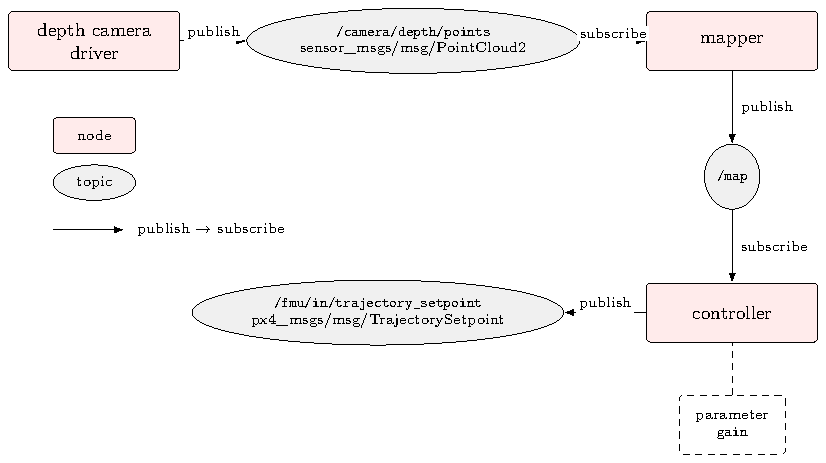
\includegraphics[width=0.9\linewidth]{figures/ros_graph}
\caption{A ROS 2 graph. Nodes never call each other: they publish to and subscribe from named, typed topics. A node can expose parameters such as a gain.}
\end{figure}

\subsection{QoS: why PX4 topics need special
settings}\label{qos-why-px4-topics-need-special-settings}

Quality of Service (QoS) settings decide how messages are delivered. A
publisher and a subscriber only connect if their settings are
\emph{compatible}. The two settings that matter here:

\begin{itemize}
\item
  \textbf{Reliability}: \emph{reliable} resends lost messages;
  \emph{best effort} does not. Sensor streams use best effort, since a
  late old sample is worse than a lost one.
\item
  \textbf{Durability}: \emph{volatile} sends only to subscribers present
  at publish time; \emph{transient local} keeps the last message for
  late subscribers.
\end{itemize}

The ROS 2 default for a subscriber is reliable and volatile. PX4 does
not use these defaults, so a default subscriber to a PX4 topic can
silently receive nothing, which is the most common beginner failure. The
PX4 documentation says subscribers ``must specify a appropriate
(compatible) QoS setting'' and uses the predefined sensor-data profile
(\texttt{rmw\_qos\_profile\_sensor\_data}: best effort, volatile, small
queue) for PX4 output topics; its example sets a depth of 5. The guide
gives no per-topic settings, so use that profile for every PX4 topic.
Publishers to \texttt{/fmu/in/} need no special QoS: the ROS 2 default
is compatible. If a subscription shows no data, check with
\texttt{ros2 topic info -v \textless{}topic\textgreater{}}, which
prints the QoS of each endpoint.

\subsection{Workspaces and colcon}\label{workspaces-and-colcon}

Your code lives in a \emph{workspace}: a folder with a \texttt{src/}
directory. \texttt{colcon} builds every package in \texttt{src/}.

\begin{lstlisting}[language=bash]
source /opt/ros/jazzy/setup.bash
cd ~/my_repo
colcon build --packages-select px4_msgs     # build one package
source install/setup.bash                   # make the result visible
\end{lstlisting}

Colcon creates \texttt{build/}, \texttt{install/} and \texttt{log/}.
Never edit them and never commit them. The order matters: first source
the ROS base install (the \emph{underlay}), then build, then source
\texttt{install/setup.bash} (the \emph{overlay}) in every new terminal
where you want to run your packages. Build only what you changed with
\texttt{-\/-packages-select}; large packages can be slow to compile.

\begin{figure}[htbp]
\centering
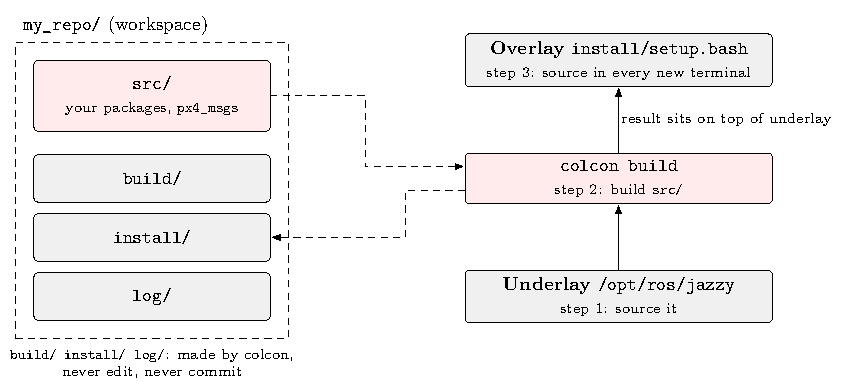
\includegraphics[width=0.9\linewidth]{figures/colcon_ws}
\caption{Your sources live in \texttt{src/}; colcon creates \texttt{build/}, \texttt{install/} and \texttt{log/}. Source the underlay, build, then source the overlay.}
\end{figure}

\subsection{Command line tools}\label{command-line-tools}

\begin{lstlisting}[language=bash]
ros2 topic list                              # all topics
ros2 topic info /fmu/out/vehicle_status -v   # type and QoS (name may differ)
ros2 topic echo <topic>                      # print messages
ros2 topic hz <topic>                        # publication rate
ros2 interface show px4_msgs/msg/TrajectorySetpoint   # message fields
ros2 node list                               # running nodes
ros2 param list /my_node                     # parameters of a node
ros2 launch <package> <file>.launch.py       # start a launch file
rqt_graph                                    # picture of nodes and topics
rviz2                                        # 3D view: clouds, maps, paths
\end{lstlisting}

Before you use a message field, check its name with
\texttt{ros2 interface show}. If two people on one network see each other's topics
by accident, set a different \texttt{ROS\_DOMAIN\_ID} (0 to 101) in each
terminal.


\begin{figure}[htbp]
\centering
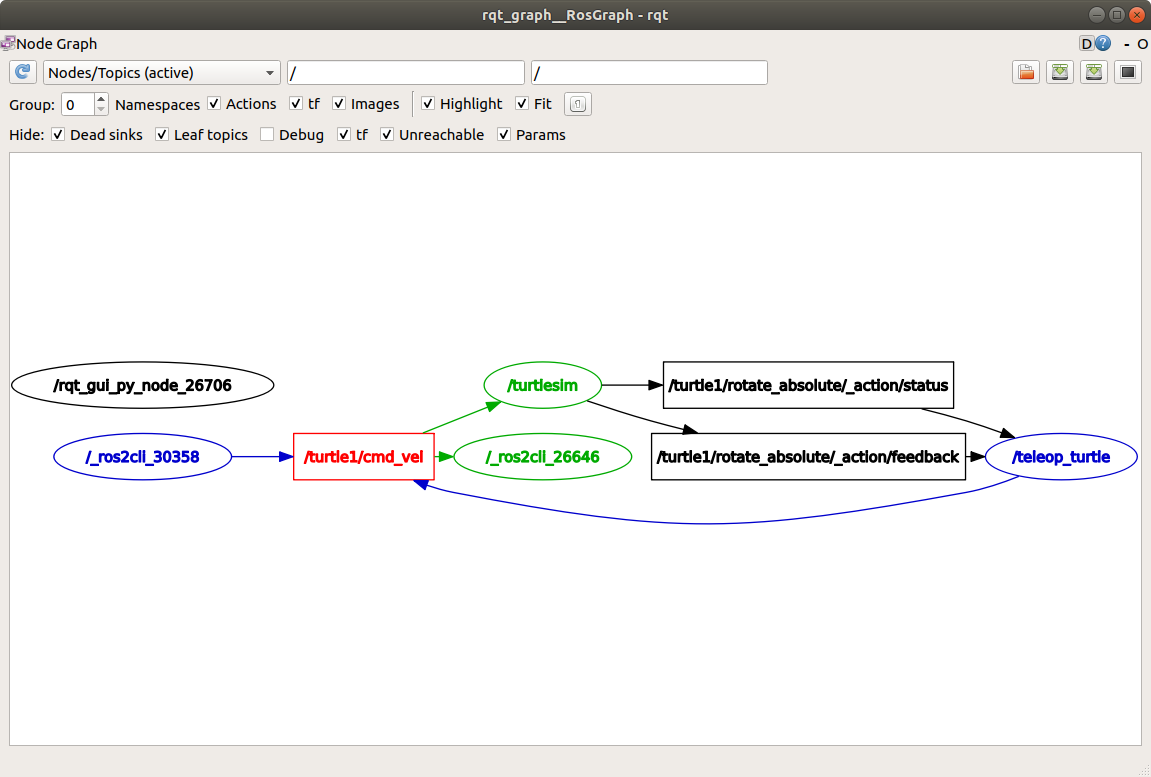
\includegraphics[width=0.8\linewidth]{figures/web/rqt_graph_turtlesim.png}
\caption{\texttt{rqt\_graph} draws the live graph: here the turtlesim nodes and the \texttt{/turtle1/cmd\_vel} topic. Image: ROS 2 Documentation (Jazzy), CC BY 4.0.}
\end{figure}

\subsection{A minimal node}\label{a-minimal-node}

A subscriber in Python (\texttt{rclpy}) that prints the north position
from PX4, with a compatible QoS. The field \texttt{x} exists in
\texttt{px4\_msgs/msg/VehicleLocalPosition}; it is the north position in
the NED frame, in metres (checked in the \texttt{msg} folder of
\texttt{px4\_msgs}). The topic name must be checked with
\texttt{ros2 topic list} (\hyperref[px4]{PX4}).

\begin{lstlisting}[language=python]
import rclpy
from rclpy.node import Node
from rclpy.qos import qos_profile_sensor_data
from px4_msgs.msg import VehicleLocalPosition

class Echo(Node):
    def __init__(self):
        super().__init__("echo")
        self.create_subscription(
            VehicleLocalPosition, "/fmu/out/vehicle_local_position",
            self.cb, qos_profile_sensor_data)

    def cb(self, msg):
        self.get_logger().info(f"north = {msg.x:.2f} m")

rclpy.init()
rclpy.spin(Echo())
\end{lstlisting}

Run it with \texttt{python3 echo.py} in a terminal where both ROS and
the workspace are sourced. C++ nodes (\texttt{rclcpp}) have the same
structure: create the node, create subscriptions and publishers, spin.

\section{PX4}\label{px4}

\subsection{Architecture}\label{architecture}

PX4 is the flight-controller firmware. It runs on the flight-controller
board (or, in simulation, as a normal program on your PC). It reads the
IMU and other sensors, estimates the vehicle state (with an EKF), and
runs the control loops that turn setpoints into motor commands. Inside
PX4, modules communicate through \textbf{uORB}, a publish/subscribe
system like ROS topics but internal to the firmware. PX4 does not run
ROS. A bridge (\hyperref[the-uxrce-dds-bridge]{uXRCE-DDS bridge}) copies
chosen uORB topics to ROS 2.

\begin{figure}[htbp]
\centering
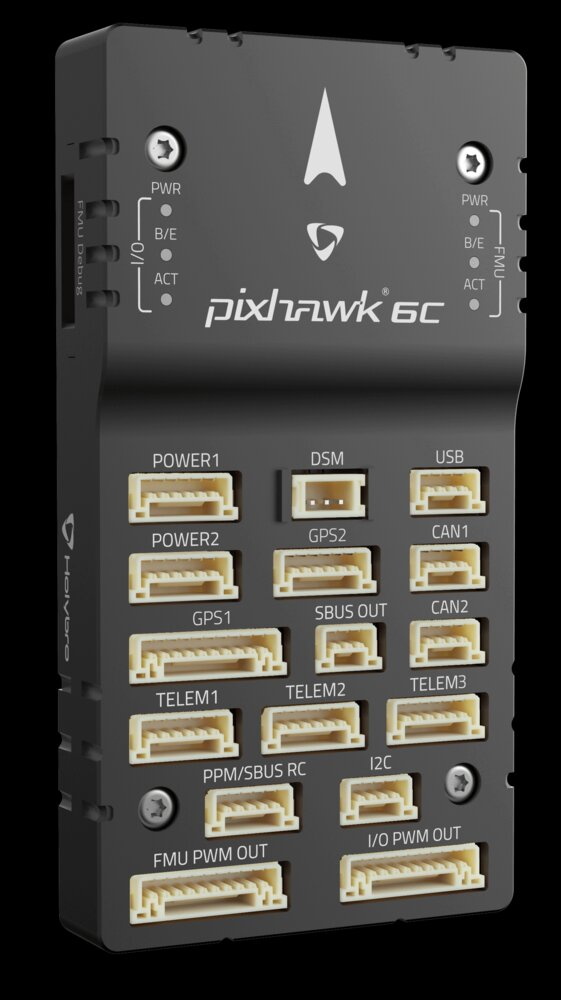
\includegraphics[width=0.38\linewidth]{figures/web/pixhawk6c_board.jpg}
\caption{A flight-controller board (Holybro Pixhawk 6C) with its ports. PX4 runs on it. Image: PX4 User Guide (Holybro), CC BY 4.0.}
\end{figure}

Control is hierarchical. Your controller outputs a setpoint, for example
an acceleration. PX4's position and velocity controllers turn it into an
attitude and thrust setpoint; the attitude and rate loops close the rest
at a much higher rate. This is why a high-level planner can often treat
the vehicle as a point mass: the fast inner loops are PX4's job.

\begin{figure}[htbp]
\centering
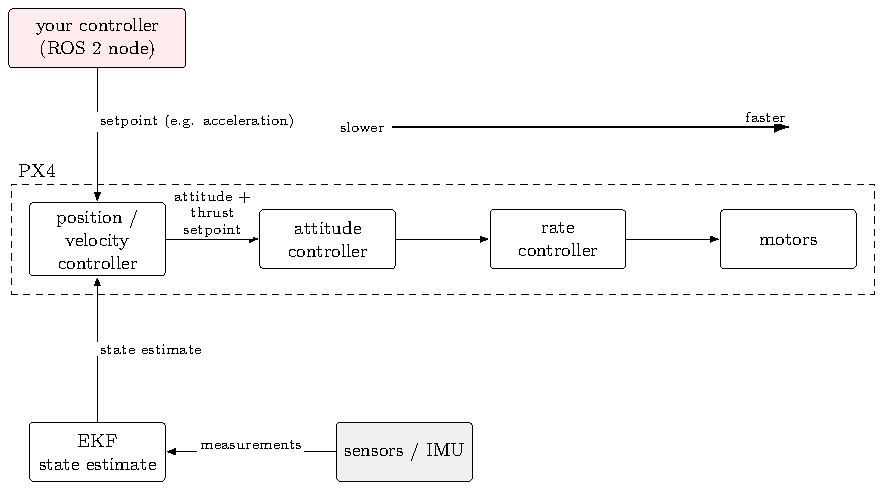
\includegraphics[width=0.95\linewidth]{figures/control_loops}
\caption{Control hierarchy. Your node sends a setpoint; PX4's position, attitude and rate loops, each faster than the last, turn it into motor commands. The EKF feeds the state estimate back to the position controller.}
\end{figure}

\subsection{Flight modes and offboard
mode}\label{flight-modes-and-offboard-mode}

A flight mode decides who produces the setpoints. Manual and stabilised
modes follow the pilot's sticks. Position mode holds position. Hold,
Return and Land are automatic. \textbf{Offboard} mode follows setpoints
that arrive from an external computer, which is your ROS 2 node.

Rules for offboard mode, from the PX4 documentation:

\begin{itemize}
\item
  PX4 must \emph{already receive} \texttt{OffboardControlMode} messages
  before it accepts offboard mode or arms in it. Start the stream first.
\item
  \texttt{OffboardControlMode} must be sent together with a setpoint
  message (for example \texttt{TrajectorySetpoint}). The first message
  says \emph{which} fields are used; the second carries the values.
\item
  If the stream of \texttt{OffboardControlMode} drops below about 2 Hz,
  PX4 leaves offboard mode (failsafe). Send both at a steady rate well
  above that. The official example uses a 100 ms timer (10 Hz); 50 Hz or
  more is common.
\item
  The official example sends 10 setpoints, then requests the mode
  switch, then arms.
\end{itemize}

\begin{figure}[htbp]
\centering
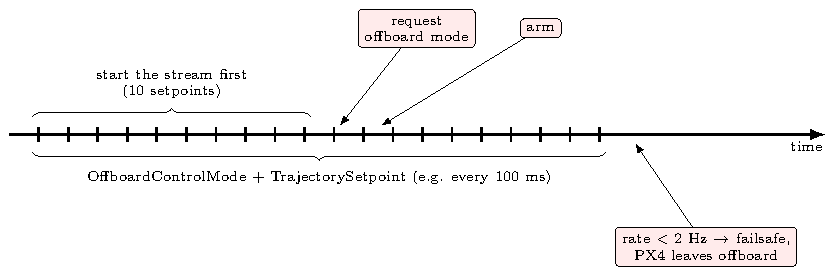
\includegraphics[width=0.9\linewidth]{figures/offboard_seq}
\caption{Offboard timeline: stream first, then request offboard mode and arm. If the stream drops below about 2\,Hz, PX4 leaves offboard mode.}
\end{figure}

The three messages (fields checked in the \texttt{msg} folder of
\texttt{px4\_msgs}):

\begin{itemize}
\item
  \texttt{OffboardControlMode}: \texttt{timestamp} and the booleans
  \texttt{position}, \texttt{velocity}, \texttt{acceleration},
  \texttt{attitude}, \texttt{body\_rate}, \texttt{thrust\_and\_torque},
  \texttt{direct\_actuator}. For acceleration control set
  \texttt{acceleration = true} and the others false.
\item
  \texttt{TrajectorySetpoint}: \texttt{timestamp},
  \texttt{position{[}3{]}}, \texttt{velocity{[}3{]}},
  \texttt{acceleration{[}3{]}}, \texttt{jerk{[}3{]}}, \texttt{yaw},
  \texttt{yawspeed}. In NED, metres and seconds. Set every field you do
  not control to NaN: the message file says NaN means ``the state should
  not be controlled''. For example, to command an acceleration, set
  \texttt{acceleration} and leave \texttt{position} and
  \texttt{velocity} NaN.
\item
  \texttt{VehicleCommand}: \texttt{command}, \texttt{param1},
  \texttt{param2}, \ldots, \texttt{target\_system},
  \texttt{target\_component}, \texttt{source\_system},
  \texttt{source\_component}, \texttt{from\_external}. Arm with the
  command \texttt{VEHICLE\_CMD\_COMPONENT\_ARM\_DISARM} (400),
  \texttt{param1 = 1}. Switch mode with
  \texttt{VEHICLE\_CMD\_DO\_SET\_MODE} (176); the official example uses
  \texttt{param1 = 1} and \texttt{param2 = 6} for offboard.
\end{itemize}

To see the current mode, read \texttt{VehicleStatus}: its
\texttt{nav\_state} equals \texttt{NAVIGATION\_STATE\_OFFBOARD} (14) and
\texttt{arming\_state} equals \texttt{ARMING\_STATE\_ARMED} (2) when all
is well.

\subsection{The uXRCE-DDS bridge}\label{the-uxrce-dds-bridge}

PX4 talks to ROS 2 through the Micro XRCE-DDS protocol. A \emph{client}
runs inside PX4 and an \emph{agent} runs on the companion computer (or
the PC in simulation). The agent exposes the PX4 topics as ROS 2 topics
under the prefix \texttt{/fmu/}: PX4 output under \texttt{/fmu/out/},
input under \texttt{/fmu/in/}. Start it for the simulator:

\begin{figure}[htbp]
\centering
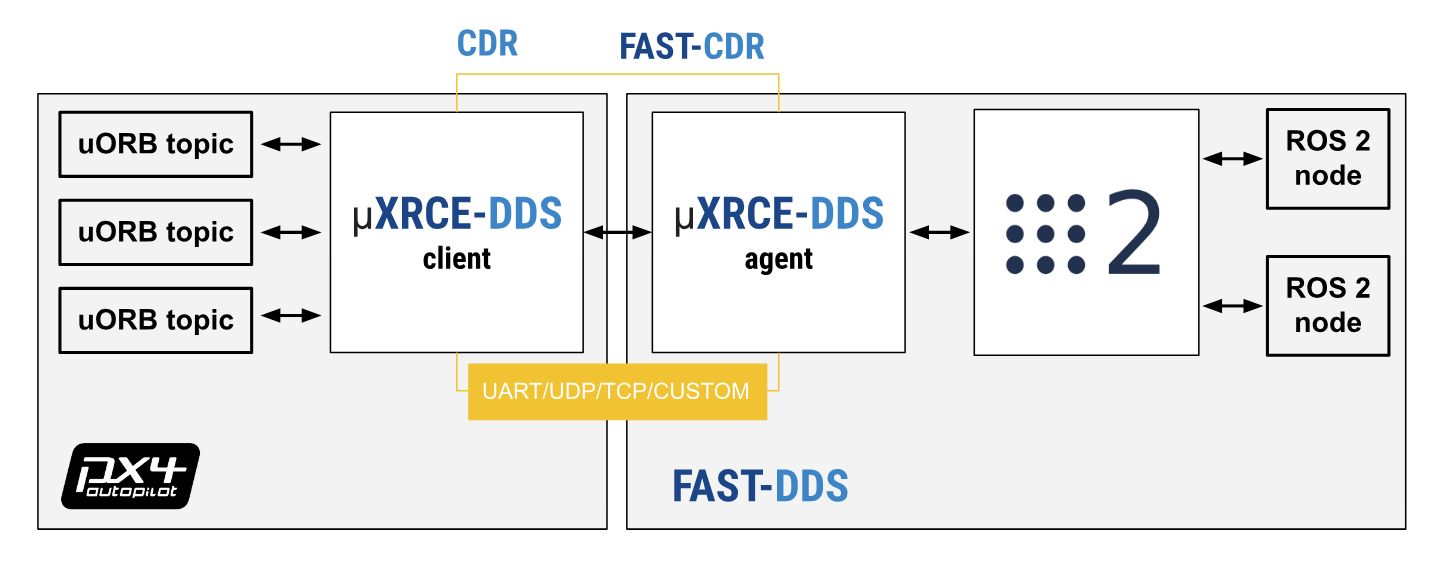
\includegraphics[width=0.9\linewidth]{figures/web/px4_uxrce_dds_architecture.png}
\caption{The uXRCE-DDS bridge: the client in PX4 talks to the agent, which exposes uORB topics as ROS 2 topics. Image: PX4 User Guide, CC BY 4.0.}
\end{figure}

\begin{lstlisting}[language=bash]
MicroXRCEAgent udp4 -p 8888
\end{lstlisting}

The PX4 ROS 2 guide uses this command. On the real drone the link
is a serial line. On our drone the agent runs as
\texttt{MicroXRCEAgent serial -\/-dev /dev/ttyTHS1 -b 921600}, and PX4
has \texttt{UXRCE\_DDS\_CFG = TELEM2} at 921600 baud. Expect names such as
\texttt{/fmu/in/offboard\_control\_mode},
\texttt{/fmu/in/trajectory\_setpoint},
\texttt{/fmu/in/vehicle\_command}. Since PX4 1.16 some messages are
versioned (the \texttt{MESSAGE\_VERSION} constant in the \texttt{.msg}
files), which may add a suffix to the topic name. Always run
\texttt{ros2 topic list} and use what you see.

\textbf{px4\_msgs must match the firmware.} The bridge sends messages as
raw binary. If the field layout in your ROS 2 package differs from the
one compiled into the firmware, data is misread or dropped. Pin
\texttt{src/px4\_msgs} to the release branch of your firmware
(\texttt{release/1.17} for PX4 1.17, see
\hyperref[submodules]{Submodules}). If the firmware changes, change the
submodule with it, and rebuild with
\texttt{colcon build -\/-packages-select px4\_msgs}.

\subsection{Frames: NED/FRD versus
ENU/FLU}\label{frames-nedfrd-versus-enuflu}

PX4 and ROS use different frame conventions, and mixing them up is the
most common source of bugs.

\begin{figure}[htbp]

\centering
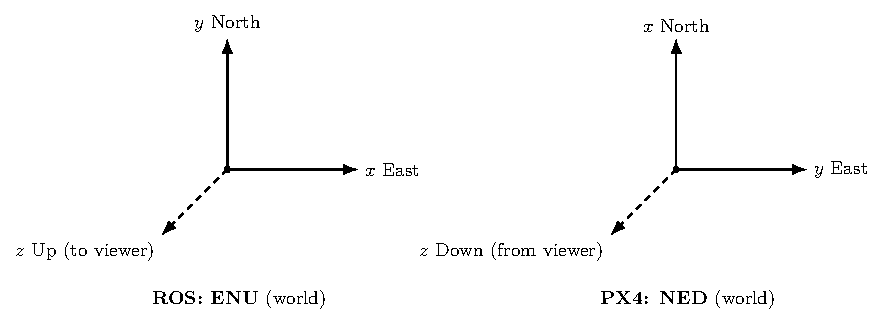
\includegraphics[width=0.9\linewidth]{figures/frames}

\caption{World frames seen from above. In ENU the third axis points up;
in NED it points down. The north and east axes swap places. Body frames
are FLU (ROS: forward, left, up) and FRD (PX4: forward, right, down).}

\end{figure}

\begin{longtable}{@{}p{0.145\linewidth} p{0.398\linewidth} p{0.398\linewidth}@{}}
\toprule
 & ROS (REP-103) & PX4 \\
\midrule
World frame & ENU: \(x\) East, \(y\) North, \(z\) Up & NED: \(x\) North,
\(y\) East, \(z\) Down \\
Body frame & FLU: \(x\) forward, \(y\) left, \(z\) up & FRD: \(x\)
forward, \(y\) right, \(z\) down \\
\bottomrule
\end{longtable}

Consequences:

\begin{itemize}
\item
  Altitude is \(-z\) in PX4. Flying 2 m above the ground means \(z=-2\)
  in the \texttt{position} of \texttt{TrajectorySetpoint} and in
  \texttt{VehicleLocalPosition.z}. A positive \(z\) setpoint drives the
  drone into the floor.
\item
  World vectors convert ENU to NED by swapping \(x\) and \(y\) and
  negating \(z\): \((x_E,y_N,z_U)\mapsto(y_N,x_E,-z_U)\). The PX4 docs
  describe it as a rotation of \(\pi/2\) about \(Z\) then \(\pi\) about
  \(X\).
\item
  Body vectors convert FLU to FRD (and back) by negating \(y\) and \(z\)
  (a rotation of \(\pi\) about \(X\)).
\item
  Yaw: PX4 yaw is measured from North, positive clockwise seen from
  above; ROS yaw is measured from East, positive counter-clockwise. A
  conversion is needed here too.
\end{itemize}

The PX4 docs recommend the helper functions in \texttt{px4\_ros\_com}
(\texttt{frame\_transforms}). Decide once, in your project, in which
frame each node works and convert only at the PX4 boundary. Many ROS
nodes use ENU internally; the setpoint is then converted to NED just
before publishing. An acceleration setpoint is a world-frame
acceleration, so the same \(x\leftrightarrow y\), \(z\to-z\) rule
applies to it.

\subsection{Simulation: SITL with
Gazebo}\label{simulation-sitl-with-gazebo}

SITL (software in the loop) runs the real PX4 firmware as a program on
your PC, with Gazebo (\texttt{gz}) simulating the drone and the world.
You need your own PX4-Autopilot checkout in
\texttt{\textasciitilde{}/PX4-Autopilot}, at tag \texttt{v1.17.0} (not
part of your project repo; see
\hyperref[installing-the-other-tools]{Installing the other tools}). The make targets from the PX4 docs are:

\begin{lstlisting}[language=bash]
cd ~/PX4-Autopilot        # path is machine-specific
make px4_sitl gz_x500                 # plain x500 quadrotor
make px4_sitl gz_x500_depth           # x500 with a front depth camera
make px4_sitl gz_x500_lidar_2d        # x500 with a 2D LiDAR
\end{lstlisting}

These three targets are listed in the PX4 Gazebo page (main
documentation). A world is chosen by appending its name to the target or
with the environment variable \texttt{PX4\_GZ\_WORLD}. The first build
takes several minutes. Simulated sensor images and point clouds reach
ROS 2 through a Gazebo-ROS bridge (package \texttt{ros\_gz\_bridge});
the topic names depend on the model.


\begin{figure}[htbp]
\centering
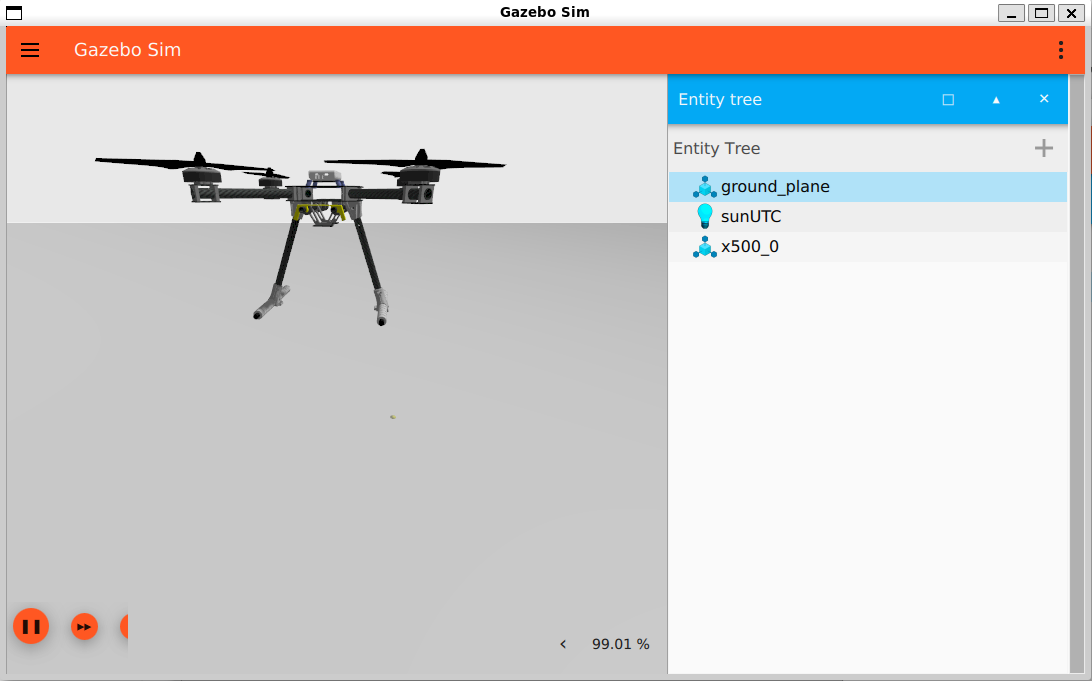
\includegraphics[width=0.85\linewidth]{figures/web/gazebo_x500_sitl.png}
\caption{Gazebo with the x500 quadrotor, as started by \texttt{make px4\_sitl gz\_x500}. Image: PX4 User Guide, CC BY 4.0.}
\end{figure}

\subsection{QGroundControl, parameters and
safety}\label{qgroundcontrol-parameters-and-safety}

\textbf{QGroundControl} (QGC) is the ground-station program. It shows
the vehicle state, lets you arm, change the flight mode, read and write
PX4 \emph{parameters}, and load failsafe settings. In simulation it
connects automatically. Parameters are named values stored in the
firmware (for example the one that enables the XRCE-DDS client). Change
them in QGC under \emph{Vehicle Setup -\textgreater{} Parameters}. Some
need a reboot. Never change a parameter on the real drone without
knowing what it does.

\begin{figure}[htbp]
\centering
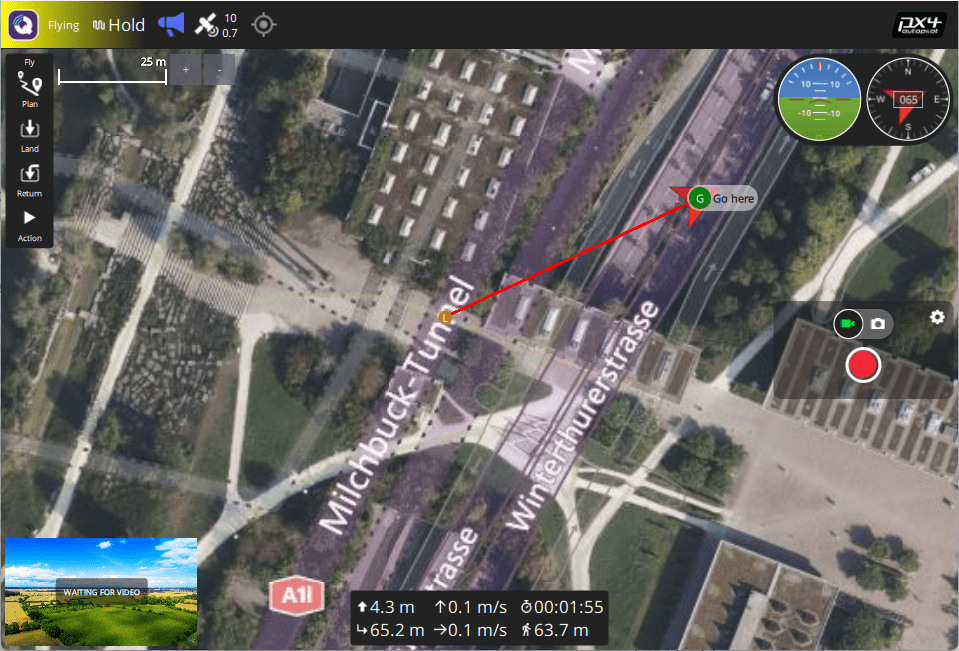
\includegraphics[width=0.85\linewidth]{figures/web/qgc_fly_view.png}
\caption{QGroundControl fly view: map, flight mode, attitude and arming. Image: PX4 User Guide, CC BY 4.0.}
\end{figure}

\begin{figure}[htbp]
\centering
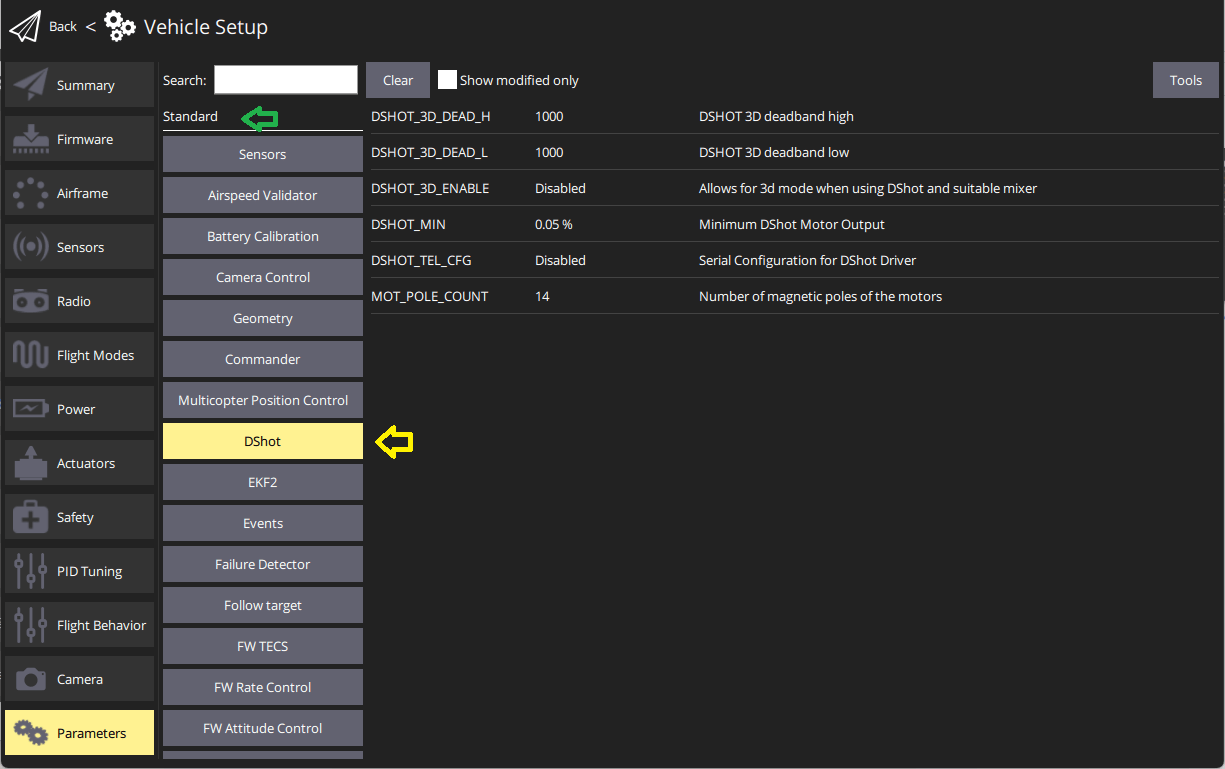
\includegraphics[width=0.85\linewidth]{figures/web/qgc_parameters.png}
\caption{QGroundControl parameter editor (\emph{Vehicle Setup -\textgreater{} Parameters}). Image: PX4 User Guide, CC BY 4.0.}
\end{figure}

\textbf{Safety in the flight cage.} Follow every rule below on every flight.

\begin{itemize}
\item
  Fly in the cage with a safety pilot holding the radio transmitter. Be
  able to leave offboard mode with one switch and take manual control.
\item
  Know the \textbf{kill switch}: it stops the motors at once. The drone
  falls. Use it only when the alternative is worse. Find its channel in
  QGC: the parameter \texttt{RC\_MAP\_KILL\_SW} shows it. Ask the safety
  pilot which physical switch that is.
\item
  Test everything in simulation first. Then fly low and slow, with props
  on only for a planned flight. Remove propellers when working on the
  bench.
\item
  If the setpoint stream stops, PX4 leaves offboard mode (see above).
  On our drone it then lands (PX4 parameter
  \texttt{COM\_OBL\_RC\_ACT}).
\end{itemize}

\section{Isaac Sim}\label{isaac-sim}

\begin{wip}
This section is a first draft. Install steps and examples will be added
once the group's Isaac Sim setup is decided.
\end{wip}

Gazebo and Isaac Sim are both simulators, used for different tasks.
Gazebo is the default simulator for PX4 and the one this guide uses
(\hyperref[simulation-sitl-with-gazebo]{Simulation: SITL with Gazebo}).
Isaac Sim is NVIDIA's simulator: it renders photorealistic cameras, so
it is better for computer vision tasks, but it requires an NVIDIA GPU.
It connects to ROS 2 through its own ROS 2 bridge.

It needs much more hardware than Gazebo. The current NVIDIA
requirements are Ubuntu 24.04 (22.04 is deprecated), an NVIDIA RTX GPU
(minimum GeForce RTX 4080, 16 GB VRAM) and 32 GB RAM. GPUs without RT
cores do not work. Check the requirements page for the version you
install.

\begin{note}
Talk to your supervisor before you install it. They will suggest a
version, a machine to run it on, and where to start (the ROS 2 bridge,
Isaac Lab or PX4 SITL). It is a large install, and the version should
match the rest of the group's setup.
\end{note}

\section{How it fits together}\label{how-it-fits-together}

\begin{figure}[htbp]

\centering
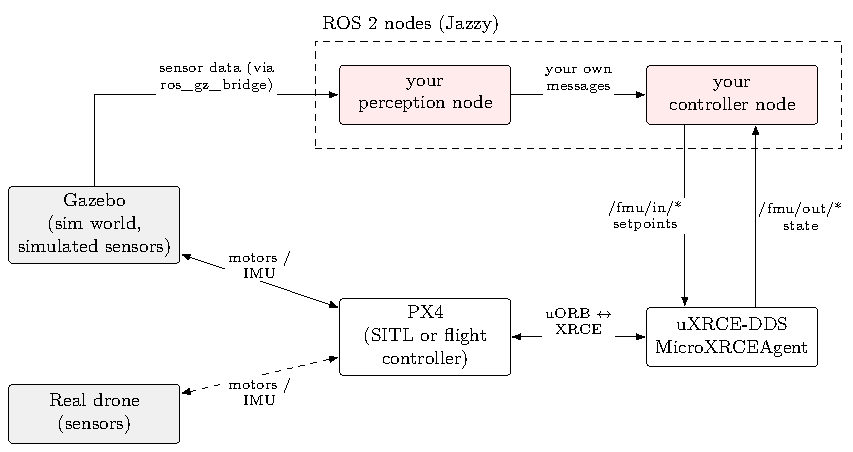
\includegraphics[width=1\linewidth]{figures/system}

\caption{Data flow. Grey: the simulator or hardware. White: PX4 and its
bridge. Red: your ROS 2 nodes. On the real drone, sensors reach your
perception node through their own ROS 2 driver (an Intel RealSense with
\texttt{realsense2\_camera}), in place of the Gazebo bridge.}

\end{figure}

The sensor produces data. Your perception node turns it into
something the controller can use. Your controller node reads the vehicle
state from PX4 (through the bridge), computes a command, and publishes
an \texttt{OffboardControlMode} and a \texttt{TrajectorySetpoint}, as in
\hyperref[px4]{PX4}, and PX4 flies it. In simulation, Gazebo plays the
part of the real world, and your nodes run the same way.

\subsection{First-day checklist}\label{first-day-checklist}

Run these one at a time and read the output. Paths in angle brackets are
yours.

\begin{checklist}
\item
  Check the system: \texttt{lsb\_release -a} (expect Ubuntu 24.04) and
  \texttt{ls /opt/ros} (expect \texttt{jazzy}). No \texttt{jazzy}?
  Install it first (\hyperref[installing-ros-2-jazzy]{Installing ROS 2
  Jazzy}).
\item
  Get GitHub access and an SSH key. Test:
  \texttt{ssh -T git@github.com}.
\item
  Clone with submodules:
  \texttt{git clone -\/-recursive git@github.com:\textless{}owner\textgreater{}/\textless{}repo\textgreater{}.git}
\item
  Check the submodules:
  \texttt{cd \textless{}repo\textgreater{} \&\& git submodule status}.
  No line may start with \texttt{-}. If one does:
  \texttt{git submodule update -\/-init -\/-recursive}.
\item
  Source ROS and build the messages:
  \texttt{source /opt/ros/jazzy/setup.bash \&\& colcon build -\/-packages-select px4\_msgs},
  then \texttt{source install/setup.bash}.
\item
  Check a message:
  \texttt{ros2 interface show px4\_msgs/msg/OffboardControlMode}.
\item
  Read the project README and the open issues on GitHub.
\item
  Set up PX4 SITL: clone PX4-Autopilot at tag \texttt{v1.17.0} into
  \texttt{\textasciitilde{}/PX4-Autopilot}
  (\hyperref[installing-the-other-tools]{Installing the other tools}),
  then in terminal 1:
  \texttt{make px4\_sitl gz\_x500}.
\item
  Terminal 2: \texttt{MicroXRCEAgent udp4 -p 8888}.
\item
  Terminal 3: source ROS and the workspace, then
  \texttt{ros2 topic list}. You should see topics under
  \texttt{/fmu/}. Check that one publishes:
  \texttt{ros2 topic hz \textless{}topic\textgreater{}}.
\item
  Open QGroundControl and check that it shows the simulated vehicle.
\item
  Hover the simulated drone in offboard mode with the example from the
  PX4 offboard control page
  (\texttt{docs.px4.io/main/en/ros2/offboard\_control.html}). Follow
  that page for how to build and run it.
\item
  Open a branch for your first task and push it:
  \texttt{git switch -c docs/1-first-day}.
\end{checklist}

\section{Further reading}\label{further-reading}

\begin{itemize}
\item
  Linux command line:
  \href{https://ubuntu.com/tutorials/command-line-for-beginners}{ubuntu.com/tutorials/command-line-for-beginners}
\item
  Pro Git book: \href{https://git-scm.com/book}{git-scm.com/book}
  (chapters 1-3 and 7.11 ``Submodules'')
\item
  GitHub docs: \href{https://docs.github.com}{docs.github.com}
\item
  ROS 2 Jazzy documentation and tutorials:
  \href{https://docs.ros.org/en/jazzy}{docs.ros.org/en/jazzy}
\item
  ROS 2 Jazzy install on Ubuntu:
  \href{https://docs.ros.org/en/jazzy/Installation/Ubuntu-Install-Debs.html}{docs.ros.org/en/jazzy/Installation/Ubuntu-Install-Debs.html}
\item
  REP-103 (units and frame conventions):
  \href{https://www.ros.org/reps/rep-0103.html}{www.ros.org/reps/rep-0103.html}
\item
  PX4 user and developer guide: \href{https://docs.px4.io}{docs.px4.io}
  (use the page for version 1.17)
\item
  PX4 ROS 2 user guide and offboard example:
  \href{https://docs.px4.io/main/en/ros2/user_guide.html}{docs.px4.io/main/en/ros2/user\_guide.html},
  \href{https://docs.px4.io/main/en/ros2/offboard_control.html}{docs.px4.io/main/en/ros2/offboard\_control.html}
\item
  PX4 Gazebo simulation:
  \href{https://docs.px4.io/main/en/sim_gazebo_gz/}{docs.px4.io/main/en/sim\_gazebo\_gz/}
\item
  Isaac Sim requirements:
  \href{https://docs.isaacsim.omniverse.nvidia.com/latest/installation/requirements.html}{docs.isaacsim.omniverse.nvidia.com/latest/installation/requirements.html}
\item
  Message definitions:
  \href{https://github.com/PX4/px4_msgs}{github.com/PX4/px4\_msgs}
\item
  Micro XRCE-DDS Agent:
  \href{https://github.com/eProsima/Micro-XRCE-DDS-Agent}{github.com/eProsima/Micro-XRCE-DDS-Agent}
\item
  QGroundControl user guide:
  \href{https://docs.qgroundcontrol.com}{docs.qgroundcontrol.com}
\item
  Gazebo: \href{https://gazebosim.org/docs}{gazebosim.org/docs}
\end{itemize}




\end{document}
